% !TEX root = ../thesis-sample.tex

\chapter{Background and Methods} \label{chap:methods}
\graphicspath{{background_methods/figs/}}


Localized surface plasmon resonance (LSPR) is an optical phenomenon generated by electromagnetic waves 
that excite the free electrons on the surface of a conductive small nanoparticle. These electrons resonate  
with the incoming electric field, forming plasmons (see Figure \ref{fig:lspr}). When resonance occurs, 
most of the incoming energy is either absorbed by the nanoparticle, or scatter in multiple directions, both
creating a large shadow behind the scatterer (a.k.a. extinction cross section). If the nanoparticle is 
smaller than $20$ nm, absorption dominates and scattering contributions are negligible \cite{PetryayevaKrull2011, OlsonETal2015}.

\begin{figure}
   \centering
     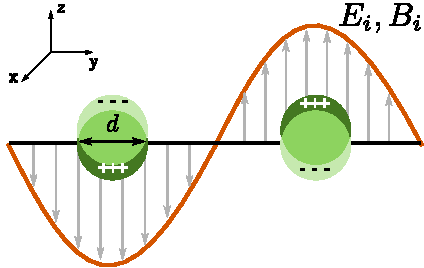
\includegraphics[width=0.55\textwidth]{lspr.pdf} 
     \caption{Illustration of the localized surface plasmon resonance (LSPR) effect of a metallic nanoparticle under an electromagnetic field.}
     \label{fig:lspr}
\end{figure}

The phenomenon of LSPR can be used for biosensing, as the resonance frequency is highly dependent on the dielectric environment 
around the scatterer. The resonance frequency shifts whenever an analyte binds to the nanoparticle, 
resulting in a very sensitive method of detecting its presence \cite{HaesVanduyne2002,HaesETal2004}
(see Figure \ref{fig:lspr_bio}). Even though LSPR is an optical effect, electrostatic theory
provides a good approximation when the wavelength of the incoming electric field is much larger than 
the size of the nanoparticle (long-wavelength limit). 

Throughout this work, we use the boundary integral electrostatic solver \pygbe \cite{ClementiETal2017} to compute 
the LSPR response of a silver nanoparticle, and how it varies in the presence of biomolecules. We treat Maxwell's equations
quasi-statically \cite{MayergoyzZhang2007} and explicitly represent the target biomolecules by a surface mesh.

\begin{figure}
   \centering
     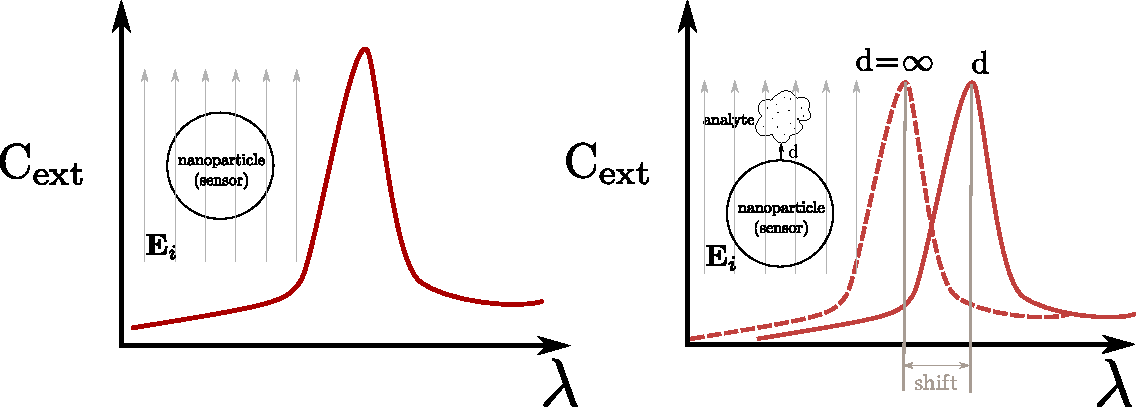
\includegraphics[width=0.95\textwidth]{lspr_biosensing.pdf} 
     \caption{Illustration of LSPR response shift in the presence of an analyte.}
     \label{fig:lspr_bio}
\end{figure}


The first implementation of \pygbe relied on continuum electrostatics to compute the solvation energy
of biomolecules. These biomolecules are modeled as dielectric cavities inside an infinite continuum 
solvent, leading to a Poisson equation inside the molecules and Laplace or Poisson-Boltzmann
(accountability of salt ions) in the solvent. The partial differential equations that model this problem
can be expressed as boundary integral equations along the molecular interface, and solved using 
\pygbe's boundary element method implementation \cite{CooperBardhanBarba2013,CooperClementiBarba2015}.
This work extends \pygbe to nanoplasmonics in the quasistatic limit for LSPR biosensing application. In the long-wavelength limit,
Maxwell's equations can be approximated by a Laplace equation, allowing us to use the methods implemented in \pygbe with modifications
to accept complex-valued permittivities, and to include the effect of an external electric field. This chapter describes the mathematical
formulation for computing electromagnetic scattering in the long-wavelength setting, and develops the associated boundary 
integral equations and their discretized form.

%%%%%EDIT
\section{Scattering of small particles} \label{sec:scattering_small}

In this section, we show how electrostatic theory is a first order approximation of Maxwell's 
equations and that it applies in the long-wavelength limit. We present the derivation from 
Mayergoyz and Zhang \cite{MayergoyzZhang2007}, due to its importance to explain the boundary 
element methods approach for our LSPR biosensor model. The following derivation considers only one particle 
in the domain, but the analysis extends to multiple particles. Figure \ref{fig:part_wave} shows a 
sketch of the system that we analyze in this derivation. Region $\Omega_1$ is a nanoparticle 
immersed in a host medium $\Omega_2$, and subjected to an incoming electromagnetic wave with  electric field 
$\mathbf{E}_i$ and magnetic field $\mathbf{B}_i$.

\begin{figure}%[h] %  figure placement: here, top, bottom, or page
   \centering
   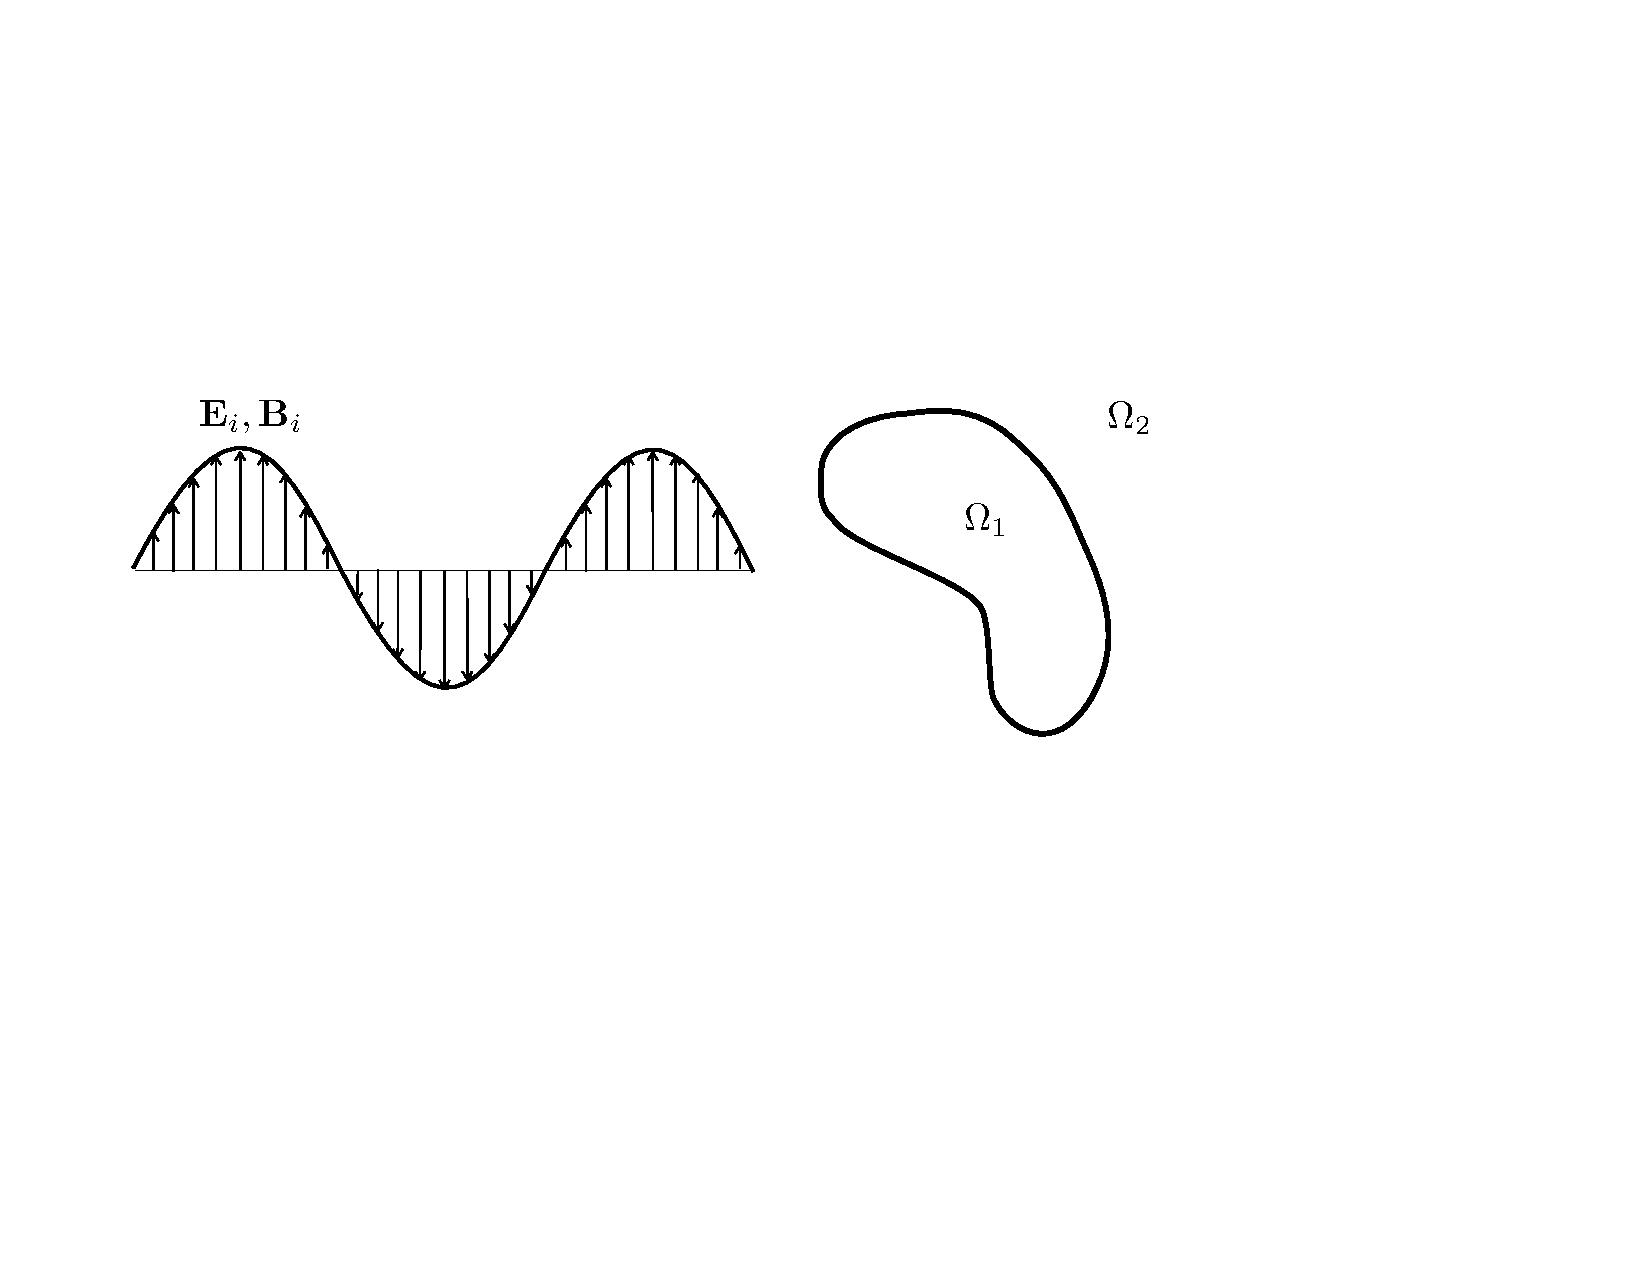
\includegraphics[width=0.65\textwidth]{particle_wave.pdf} 
   \caption{Nanoparticle interacting with an electromagnetic wave.}
   \label{fig:part_wave}
\end{figure}


Equation \eqref{eq:maxwell_timeharmonic} is a system of partial differential equations that
models a scattered, time-harmonic electromagnetic field. Where the electric field $\mathbf{E}$ and 
the magnetic field $\mathbf{B} = \mu \mathbf{H}$ vary only in space. 

\begin{align} \label{eq:maxwell_timeharmonic}
   \epsilon_1 \nabla \cdot \mathbf{E}_{1s} =& \rho_{f1} \qquad \nabla \times \mathbf{E}_{1s} = -\mu_1i\omega\mathbf{H}_{1s} \nonumber \\
   \mu_1\nabla \cdot \mathbf{H}_{1s} =& 0 \qquad \nabla \times \mathbf{H}_{1s} = \mathbf{J}_{f1} + \epsilon_1i\omega\mathbf{E}_{1s} + (\epsilon_1-\epsilon_2)i\omega\mathbf{E}_{i}\qquad \text{ on $\Omega_1$,} \nonumber \\
   \epsilon_2 \nabla \cdot \mathbf{E}_{2s} =& \rho_{f2} \qquad \nabla \times \mathbf{E}_{2s} = -\mu_2i\omega \mathbf{H}_{2s} \nonumber \\
   \mu_2\nabla \cdot \mathbf{H}_{2s} =& 0 \qquad \nabla \times \mathbf{H}_{2s} = \mathbf{J}_{f2} + \epsilon_2i\omega\mathbf{E}_{2s} \qquad \text{ on $\Omega_2$, and} \nonumber \\
   (\epsilon_1\mathbf{E}_{1s}-\epsilon_2\mathbf{E}_{2s})&\cdot\mathbf{n} = (\epsilon_2-\epsilon_1)\mathbf{E}_i\cdot\mathbf{n} \nonumber \\
   \mathbf{H}_{1s}&\cdot \mathbf{n} = \mathbf{H}_{2s}\cdot\mathbf{n} \qquad\text{ on the interface $\Gamma$}.
\end{align} 

In a setting with no charges or currents like in Figure \ref{fig:part_wave}, Equation \eqref{eq:maxwell_timeharmonic} becomes
 %
 \begin{align} \label{eq:maxwell_nocharge}
 \nabla \cdot \mathbf{E}_{1s} &= 0 \qquad \nabla \times \mathbf{E}_{1s} = -\mu_1i\omega\mathbf{H}_{1s} \nonumber \\
 \nabla \cdot \mathbf{H}_{1s} &= 0 \qquad \nabla \times \mathbf{H}_{1s} = \epsilon_1i\omega\mathbf{E}_{1s} + (\epsilon_1-\epsilon_2)i\omega\mathbf{E}_{i} \qquad \text{on $\Omega_1$} \nonumber \\
 \nabla \cdot \mathbf{E}_{2s} &= 0 \qquad \nabla \times \mathbf{E}_{2s} = -\mu_2i\omega\mathbf{H}_{2s} \nonumber \\
 \nabla \cdot \mathbf{H}_{2s} &= 0 \qquad \nabla \times \mathbf{H}_{2s} = \epsilon_2i\omega\mathbf{E}_{2s} \qquad \text{on $\Omega_2$} \nonumber \\
 (\epsilon_1\mathbf{E}_{1s} - \epsilon_2\mathbf{E}_{2s})\cdot\mathbf{n} &= (\epsilon_2-\epsilon_1)\mathbf{E}_i\cdot \mathbf{n} \nonumber \\(\mathbf{H}_{1s} - \mathbf{H}_{2s})\cdot \mathbf{n}&=0 \qquad \text{on the interface $\Gamma$,}
 \end{align}
 
 We want to study the effect of the size of the particle in the scattered field, to do so we need 
 to use the following scaled quantities:
 %
 \begin{align}\label{eq:scaled_quant}
 \mathbf{e}_i = \sqrt{\epsilon_2}\mathbf{E}_i, \qquad \mathbf{e}_s = \sqrt{\epsilon_2}\mathbf{E}_s, \nonumber \\
 \mathbf{h}_s = \sqrt{\mu_2}\mathbf{H}_s \qquad \mathbf{x}^\prime = \frac{\mathbf{x}}{d},
 \end{align}
 
 where $d$ is the particle size, and $\mathbf{x}^\prime$ a scaled domain. Turning
 Equation \eqref{eq:scaled_quant} into Equation \eqref{eq:maxwell_nocharge}, we get
 %
 \begin{align} \label{eq:maxwell_scaled}
 \nabla \cdot \mathbf{e}_{1s} &= 0 \qquad \nabla \times \mathbf{e}_{1s} = -i\beta\mathbf{h}_{1s}\frac{\mu_1}{\mu_2} \nonumber \\
 \nabla \cdot \mathbf{h}_{1s} &= 0 \qquad \nabla \times \mathbf{h}_{1s} = \frac{\epsilon_1-\epsilon_2}{\epsilon_2}i\beta\mathbf{e}_{i}+\frac{\epsilon_1}{\epsilon_2}i\beta\mathbf{e}_{1s}  \qquad \text{on $\Omega_1$} \nonumber \\
 \nabla \cdot \mathbf{e}_{2s} &= 0 \qquad \nabla \times \mathbf{e}_{2s} = -i\beta\mathbf{h}_{2s} \nonumber \\
 \nabla \cdot \mathbf{h}_{2s} &= 0 \qquad \nabla \times \mathbf{h}_{2s} = i\beta\mathbf{e}_{2s} \qquad \text{on $\Omega_2$} \nonumber \\
 (\epsilon_1\mathbf{e}_{1s} - \epsilon_2\mathbf{e}_{2s})\cdot\mathbf{n} &= (\epsilon_2-\epsilon_1)\mathbf{e}_i\cdot \mathbf{n} \nonumber \\(\mathbf{h}_{1s} - \mathbf{h}_{2s})\cdot \mathbf{n}&=0 \qquad \text{on the interface $\Gamma$,}
 \end{align}
 
 with $\beta=\omega d \sqrt{\epsilon_2\mu_2}$. We can expand $\mathbf{e}$ and $\mathbf{h}$ in 
 terms of $\beta$ as
 %
 \begin{align} \label{eq:expand}
 \mathbf{e} &= \mathbf{e}_s^{(0)} + \beta \mathbf{e}_s^{(1)} + \beta^2 \mathbf{e}_s^{(2)} + \ldots \nonumber\\
 \mathbf{h} &= \mathbf{h}_s^{(0)} + \beta \mathbf{h}_s^{(1)} + \beta^2 \mathbf{h}_s^{(2)} + \ldots,
 \end{align}
 
 If we consider only the zeroth order terms in Equation \eqref{eq:maxwell_scaled} we get
 %
 \begin{align} \label{eq:maxwell_scatter_zeroth}
 \nabla \cdot \mathbf{e}^{(0)}_{1s} &= 0 \qquad \nabla \times \mathbf{e}^{(0)}_{1s} = 0 \nonumber \\
 \nabla \cdot \mathbf{h}^{(0)}_{1s} &= 0 \qquad \nabla \times \mathbf{h}^{(0)}_{1s} = 0 \nonumber \\
 \nabla \cdot \mathbf{e}^{(0)}_{2s} &= 0 \qquad \nabla \times \mathbf{e}^{(0)}_{2s} = 0 \nonumber \\
 \nabla \cdot \mathbf{h}^{(0)}_{2s} &= 0 \qquad \nabla \times \mathbf{h}^{(0)}_{2s} = 0 \nonumber \\
 (\epsilon_1\mathbf{e}^{(0)}_{1s} - \epsilon_2\mathbf{e}^{(0)}_{2s})\cdot\mathbf{n} &= (\epsilon_2-\epsilon_1)\mathbf{e}_i\cdot \mathbf{n} \nonumber \\(\mathbf{h}^{(0)}_{1s} - \mathbf{h}^{(0)}_{2s})\cdot \mathbf{n}&=0.
 \end{align}

Equation \eqref{eq:maxwell_scatter_zeroth} has the form of an electrostatic field, where the electric
and magnetic fields are decoupled. Then $\mathbf{h}^{(0)}=0$ and $\mathbf{e}^{(0)}$ can be described by a
scalar potential since $\nabla \times \mathbf{e}^{(0)}=0$.
 
Equation \eqref{eq:maxwell_scatter_zeroth} is a good approximation as long as $\beta$ is small. On the host medium, the wave 
speed is $c=1/\sqrt{\epsilon_2\mu_2}$, then $\beta=\omega d \sqrt{\epsilon_2\mu_2} = d\omega/c  = d/\lambda$. In this work
we look at the long-wavelength limit ($\lambda > d$), that translates in Equation \eqref{eq:maxwell_scatter_zeroth} becoming
a valid approximation, making electrostatic theory suitable to model localized surface plasmon resonance (quasi-static approximation).

In Equation \eqref{eq:maxwell_scatter_zeroth}, the zeroth order term of the magnetic field is zero
everywhere, therefore we will concentrate only on the electric field. Ignoring all the terms related 
to the magnetic field, we can rewrite Equation \eqref{eq:maxwell_scatter_zeroth} in terms of 
$\mathbf{E}$ and $\mathbf{x}$ instead of the scaled quantities $\mathbf{e}$ and
$\mathbf{x}^\prime$, as:

\begin{align} \label{eq:electrostatic_scatter_E}
\nabla \cdot \mathbf{E}_{1s} &= 0 \qquad \nabla \times \mathbf{E}_{1s} = 0, \nonumber \\
\nabla \cdot \mathbf{E}_{2s} &= 0 \qquad \nabla \times \mathbf{E}_{2s} = 0, \nonumber \quad
\text{with interface conditions, } \nonumber \\
(\epsilon_1\mathbf{E}_{1s} &- \epsilon_2\mathbf{E}_{2s})\cdot\mathbf{n} = (\epsilon_2-\epsilon_1)\mathbf{E}_i\cdot \mathbf{n}.
\end{align}

In Equation \eqref{eq:electrostatic_scatter_E}, $\mathbf{E}_{1s}$ and $\mathbf{E}_{2s}$ 
are the electric fields of the scattered wave in the nanoparticle and host regions, respectively 
(see Figure \ref{fig:part_wave}), $\mathbf{E}_{i}$ is the electric field of the incoming wave, and $\epsilon_1$ 
and $\epsilon_2$ are the permittivities. This approximation decouples the electric and magnetic fields, neglects the magnetic field, 
and describes the electric field as a curl-free vector field. Hence, we can reformulate Equation \eqref{eq:electrostatic_scatter_E} with a scalar potential
($-\nabla \phi_{js} = \mathbf{E}_{js}$), as follows:
%
\begin{align} \label{eq:electrostatic_scatter}
\nabla^2 \phi_{1s} &= 0 \qquad \nabla^2 \phi_{2s} = 0 \qquad\text{on $\Omega_1$, $\Omega_2$} \nonumber \\
\epsilon_1\frac{\partial\phi_{1s}}{\partial \mathbf{n}} - \epsilon_2\frac{\partial\phi_{2s}}{\partial\mathbf{n}} &= (\epsilon_2-\epsilon_1)\frac{\partial\phi_i}{\partial\mathbf{n}} \quad \phi_{1s} = \phi_{2s} \quad \text{on $\Gamma$}.
\end{align}
%
Equation \eqref{eq:electrostatic_scatter} is an electrostatic equation with an imposed electric
field $\mathbf{E}_i=-\nabla\phi_i$, where $\Gamma$ is the boundary between the regions $\Omega_1$ and $\Omega_2$.

\subsection{Far-field scattering} \label{sec:ff_scattering}

In LSPR, the scattered electromagnetic wave is measured by a detector located far away 
from the scatterer (nanoparticle), and the plasmon resonance is identified when the energy 
detected is minimum. In the far-field limit, the scattered field
in the outside region ($\Omega_2$) is given by: 

\begin{equation} \label{eq:scat_efield_long_range}
    \mathbf{E}_{2s} = \frac{1}{4\pi\epsilon_2}k^2\frac{e^{ikr}}{r} (\mathbf{\hat{r}} \times \mathbf{p})\times\mathbf{\hat{r}}.
\end{equation} 

where $k=2\pi/\lambda$ is the wave number and $\lambda$ the wavelength, $\mathbf{\hat{r}}$ 
is a unit vector in the direction of the observation point, and $\mathbf{p}$ is
the dipole moment. 
The scattered electric field in the long wavelength limit, can also be expressed in terms of the 
scattering amplitude $\mathbf{F}$ \cite{Jackson} as:

\begin{equation} \label{eq:scat_efield_fwa}
    \mathbf{E}_{2s}(\mathbf{r})_{r\to\infty} = \frac{e^{ikr}}{r} \mathbf{F}(\mathbf{k},\mathbf{k}_0),
\end{equation}

where $\mathbf{k}$ is the scattered wave vector in the direction of propagation, and $\mathbf{k}_0$ the 
wave vector of the incident field. 

\subsection{Extinction cross-section and optical theorem} \label{sec:cext_ot}

The extinction cross-section ($C_\text{ext}$) is a measure of the energy that 
does not reach the detector, either because it is scattered in other directions,
or due to absorption. This quantity is defined as the ratio between the lost energy and 
the intensity of the incoming wave, and has units of area. The extinction cross-section peaks when
plasmons of the nanoparticle resonate with the incoming electric field.

The optical theorem connects the extinction cross section with the forward-scattering amplitude. The traditional 
expression for this relationship applies for non-absorbing media 
\cite{MayergoyzZhang2007, Jackson}; Mishchenko \cite{Mishchenko2007} corrected it for absorbing media, 
giving an expression that can be rewritten using Jackson's notation \cite{Jackson} as follows:

\begin{equation} \label{eq:cext_fwa}
    C_\text{ext} = \frac{4\pi}{k^\prime} \operatorname{Im} \left[ \frac{\mathbf{\hat{e}}_i}{|\mathbf{E}_i|}\mathbf{F}(\mathbf{k}=\mathbf{k}_0, \mathbf{k}_0) \right].
\end{equation}

where $k^\prime$ is the real part of the complex wave number, 

\begin{equation}
    k = k^\prime + ik^{\prime\prime} = \frac{2\pi}{\lambda} n,
\end{equation}

and $n$ is the refraction index of the host medium.

Combining Equations \eqref{eq:scat_efield_long_range} and \eqref{eq:scat_efield_fwa},
we can compute the scattering amplitude to  obtain the extinction cross-section 
with Equation \eqref{eq:cext_fwa}.

\section{The Boundary Element Method} \label{sec:lspr_bem}

In the context of PDEs when the differential operator has a fundamental solution and it can be expressed as a boundary integral equation (BIE), we can solve 
this BIE numerically using the boundary element method (\bem). The idea of representing partial differential equations (PDEs) as boundary integral 
equations originated in the late 1800s and early 1900s and it is documented in the work of Betti, Somigliana and Fredholm \cite{Betti1872,Somigliana1885,Fredholm1903},
which were inspired on the earlier work of Green \cite{Green1828}. The work of Fredholm is considered the starting point of the boundary element method, 
since he was the first one in compute boundary data in a potential theory application, where he used analytical techniques valid for simple geometries. Later in 
the early 1960s appeared the first numerical solution to Fredholm's equation for two dimensional potential theory \cite{Jawson1963,Symm1963}, and in the late 1960s 
for two- and three-dimensional potential theory and elasticity \cite{Rizzo1967,Cruse1969}. Since then, the boundary element method has evolved and been used 
as a numerical technique in multiple areas\cite{Atkinson1997,McLean2000,Steinbach2008, BrebbiaDominguez1992, Katsikadelis2002}. 


\subsection{Integral formulation of the Laplace equation} \label{ssec:int_form}

A well known PDE that we can solve with \bem is the Laplace equation. For a scalar quantity $\phi$ in a domain $\Omega$ with boundary $\Gamma$, and 
boundary conditions $\phi_0$ or $\partial \phi_0/\partial \mathbf{n}$, the Laplace equation takes the form:
%
\begin{align} \label{eq:lap_pde}
\nabla^2\phi &= 0 \quad \text{ on $\Omega$} \nonumber \\
\phi = \phi_0 \text{ or } \frac{\partial \phi}{\partial \mathbf{n}} &= \frac{\partial \phi_0}{\partial \mathbf{n}} \quad \text{ on $\Gamma$} 
\end{align}

The weak formulation of Laplace equation \eqref{eq:lap_pde} with test function $w$ is:

\begin{equation} \label{eq:lap_weak}
\int_\Omega \nabla^2 \phi(\mathbf{r}_\Omega') w(\mathbf{r}_\Omega') \text{d} \Omega^\prime= 0.
\end{equation}

where the evaluation point is $\mathbf{r}_\Omega$ a location in the domain $\Omega$.

If we use the Laplace's free-space Green's function as the test function $w$ we
get:

\begin{equation} \label{eq:lap_weak2}
\int_\Omega \nabla^2 \phi(\mathbf{r}'_\Omega) G_L(\mathbf{r}_\Omega,\mathbf{r}'_\Omega) \text{d} \Omega^\prime= 0.
\end{equation}

Manipulating the integrand using the product rule and later the divergence 
theorem, we get:

\begin{equation} \label{eq:lap_bie_dom}
\phi(\mathbf{r}_\Omega) = \oint_\Gamma G_L(\mathbf{r}_\Omega,\mathbf{r}'_\Gamma)  \frac{\partial} {\partial \mathbf{n}} \phi(\mathbf{r}'_\Gamma)  \text{d} \Gamma^\prime - \oint_\Gamma \phi(\mathbf{r}'_\Gamma)  \frac{\partial}{\partial \mathbf{n}} G_L(\mathbf{r}_\Omega,\mathbf{r}'_\Gamma) \text{d} \Gamma^\prime
\end{equation}

where \eqref{eq:lap_bie_dom}, $\mathbf{r}$ can be anywhere in the domain $\Omega$, 
and $\mathbf{r}'$ runs only on the boundary $\Gamma$. This equation has a 
singularity when $\mathbf{r}=\mathbf{r}'$. To handle this problem, we perform the
integral on a surface $\Gamma'$ that is like $\Gamma$ but with a hemisphere of 
radius $\varepsilon$ center at $\mathbf{r}$. We split the integrals into the part
that has no singularity and the part that has the hemisphere. After solving these
equations when $\varepsilon \to 0$, equation \eqref{eq:lap_bie_dom} results in:

\begin{equation} \label{eq:lap_bie}
\frac{\phi(\mathbf{r}_\Gamma)}{2} +  \oint_\Gamma \phi(\mathbf{r}'_\Gamma)  \frac{\partial}{\partial \mathbf{n}} G_L(\mathbf{r}_\Gamma,\mathbf{r}'_\Gamma) \text{d} \Gamma^\prime = \oint_\Gamma G_L(\mathbf{r}_\Gamma,\mathbf{r}'_\Gamma)  \frac{\partial} {\partial \mathbf{n}} \phi(\mathbf{r}'_\Gamma)  \text{d} \Gamma^\prime,
\end{equation}

where the integrals are Cauchy principal value integrals.

Using the single and double layer operators:

\begin{equation}\label{eq:single_layer}
   V^{\Gamma}_L (\psi(\mathbf{r}_\Gamma)) = \oint_\Gamma \psi(\mathbf{r}'_\Gamma) G_L(\mathbf{r}_\Gamma, \mathbf{r}'_\Gamma) \text{d} \Gamma',
   \end{equation}
   %
   \begin{equation}\label{eq:double_layer}
   K^{\Gamma}_L (\psi(\mathbf{r}_\Gamma)) = \oint_\Gamma \psi(\mathbf{r}'_\Gamma) \frac{\partial}{\partial \mathbf{n}}G_L(\mathbf{r}_\Gamma, \mathbf{r}'_\Gamma) \text{d} \Gamma'.
   \end{equation}
   %
where $G_L$ is the free-space Green's function of the Laplace equation:
   %
   \begin{equation}
   G_L(\mathbf{r},\mathbf{r}') = \frac{1}{4\pi|\mathbf{r}-\mathbf{r}'|}
   \end{equation}
   

We can rewrite equation \eqref{eq:lap_bie} using the operator notation, as:

\begin{equation} \label{eq:lap_operator}
\left[ \frac{\mathbb{I}}{2} + K_L^{\mathbf{r}_\Gamma} \right] \left( \phi_\Gamma \right) = V_L^{\mathbf{r}_\Gamma} \left( \frac{\partial}{\partial \mathbf{n}} \phi_\Gamma \right),
\end{equation}

where $\mathbb{I}$ is the identity operator.

\subsubsection{Electrostatic potential of a nanoparticle under an electric field} \label{sec:pot_elec_field}

Following the same steps from section \ref{ssec:int_form}  we can write the system of partial differential equations 
in Equation \eqref{eq:electrostatic_scatter} as a system of boundary integral equations \cite{BrebbiaDominguez1992}. Evaluating on the
surface $\Gamma$, this becomes
%
\begin{align} \label{eq:integral_eq_lspr_nobc}
\frac{\phi_{1s,\Gamma}}{2}+ K_{L}^{\Gamma}(\phi_{1s,\Gamma}) - V_{L}^{\Gamma} \left(\frac{\partial}{\partial \mathbf{n}}\phi_{1s,\Gamma} \right) = 0&  \nonumber \\
\frac{\phi_{2s,\Gamma}}{2} - K_{L}^{\Gamma}(\phi_{2s,\Gamma}) + V_{L}^{\Gamma} \left( \frac{\partial}{\partial \mathbf{n}} \phi_{2s,\Gamma} \right) = 0&,
\end{align}
%
where $V$ and $K$ are the single- and double-layer operators.
%
Applying the interface conditions of Equation \eqref{eq:electrostatic_scatter},
leads to:

\begin{align} \label{eq:integral_eq_lspr}
\frac{\phi_{1s,\Gamma}}{2}+ K_{L}^{\Gamma}(\phi_{1s,\Gamma}) - V_{L}^{\Gamma} \left(\frac{\partial}{\partial \mathbf{n}}\phi_{1s,\Gamma} \right) &= 0  \nonumber \\
\frac{\phi_{1s,\Gamma}}{2} - K_{L}^{\Gamma}(\phi_{1s,\Gamma}) + \frac{\epsilon_1}{\epsilon_2}V_{L}^{\Gamma} \left( \frac{\partial}{\partial \mathbf{n}} \phi_{1s,\Gamma}  \right) &=
 \frac{\epsilon_2-\epsilon_1}{\epsilon_2}V_{L}^{\Gamma}\left( \frac{\partial}{\partial \mathbf{n}} \phi_{i,\Gamma} \right)\quad \text{on $\Gamma$.}
\end{align}


\subsubsection{Analyte-sensor electrostatic potential under an electric field}

The sketch in Figure \ref{fig:analyte-sensor} shows a metallic nanoparticle ($\Omega_1$) interacting with an analyte ($\Omega_3$), under an external electric field.
Mathematically, this situation can be modeled as:

\begin{align}\label{eq:electrostatic_scatter_prot_sen}
\nabla^2 \phi_{1s} &= 0, \qquad \nabla^2 \phi_{2s} = 0 \qquad\text{on $\Omega_1$, $\Omega_2$} \nonumber\\
\nabla^2 \phi_{3s} &= -\frac{1}{\epsilon_3} \sum_{k=0}^{N_q} \delta(|\mathbf{r}-\mathbf{r}_k|) q_k \qquad\text{on $\Omega_3$} \nonumber \\
\epsilon_1\frac{\partial\phi_{1s}}{\partial \mathbf{n}} - \epsilon_2\frac{\partial\phi_{2s}}{\partial\mathbf{n}} &= (\epsilon_2-\epsilon_1)\frac{\partial\phi_i}{\partial\mathbf{n}} \quad \phi_{1s} = \phi_{2s} \quad \text{on $\Gamma_1$}. \nonumber\\
\epsilon_3\frac{\partial\phi_{3s}}{\partial \mathbf{n}} - \epsilon_2\frac{\partial\phi_{2s}}{\partial\mathbf{n}} &= (\epsilon_2-\epsilon_3)\frac{\partial\phi_i}{\partial\mathbf{n}} \quad \phi_{3s} = \phi_{2s} \quad \text{on $\Gamma_2$}.
\end{align}
%
where $q_k$ are the point charges of the atoms inside the protein, located at $\mathbf{r}_k$.

\begin{figure}%[b] %  figure placement: here, top, bottom, or page
   \centering
   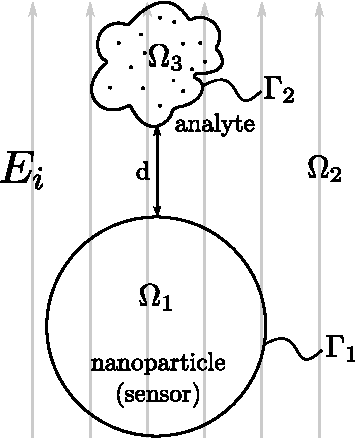
\includegraphics[width=0.35\textwidth]{protein_sensor_regions.pdf} 
   \caption{Analyte-sensor system under electric field.}
   \label{fig:analyte-sensor}
\end{figure}

Similar to Equation \eqref{eq:integral_eq_lspr}, we can write the system of partial differential equations in 
\eqref{eq:electrostatic_scatter_prot_sen} as:

\begin{align} \label{eq:integral_eq_lspr_nobc_system}
\frac{\phi_{1s,\Gamma_1}}{2}+ K_{L,\Gamma_1}^{\Gamma_1}(\phi_{1s,\Gamma_1}) &- V_{L,\Gamma_1}^{\Gamma_1} \left(\frac{\partial}{\partial \mathbf{n}}\phi_{1s,\Gamma_1} \right) = 0  \nonumber \\
\frac{\phi_{2s,\Gamma_1}}{2} - K_{L,\Gamma_1}^{\Gamma_1}(\phi_{2s,\Gamma_1}) + V_{L,\Gamma_1}^{\Gamma_1} \left(\frac{\partial}{\partial \mathbf{n}}\phi_{2s,\Gamma_1} \right) 
& - K_{L,\Gamma_2}^{\Gamma_1}(\phi_{2s,\Gamma_2}) + V_{L,\Gamma_2}^{\Gamma_1} \left(\frac{\partial}{\partial \mathbf{n}}\phi_{2s,\Gamma_2} \right) = 0  \nonumber \\
\frac{\phi_{2s,\Gamma_2}}{2} - K_{L,\Gamma_1}^{\Gamma_2}(\phi_{2s,\Gamma_1}) + V_{L,\Gamma_1}^{\Gamma_2} \left(\frac{\partial}{\partial \mathbf{n}}\phi_{2s,\Gamma_1} \right)  
&- K_{L,\Gamma_2}^{\Gamma_2}(\phi_{2s,\Gamma_2}) + V_{L,\Gamma_2}^{\Gamma_2} \left(\frac{\partial}{\partial \mathbf{n}}\phi_{2s,\Gamma_2} \right) = 0  \nonumber \\
\frac{\phi_{3s,\Gamma_2}}{2} + K_{L,\Gamma_2}^{\Gamma_2}(\phi_{3s,\Gamma_2}) &- V_{L,\Gamma_2}^{\Gamma_2} \left( \frac{\partial}{\partial \mathbf{n}} \phi_{3s,\Gamma_2} \right) = \frac{1}{4\pi\epsilon_3} \sum_{k=0}^{N_q} \frac{q_k}{|\mathbf{r}_{\Gamma_2} - \mathbf{r}_k|} ,
\end{align}
%
where $V$ and $K$ are the single- and double-layer operators in equations 
\eqref{eq:single_layer} and \eqref{eq:double_layer}. In this case, we distinguish between the
surface where the integrals run (subindex), and the surface that contains the evaluation point (superindex).

Applying the interface conditions of equation \eqref{eq:electrostatic_scatter_prot_sen},
leads to: 

\begin{align} \label{eq:integral_eq_lspr_system}
\frac{\phi_{1s,\Gamma_1}}{2}&+ K_{L,\Gamma_1}^{\Gamma_1}(\phi_{1s,\Gamma_1}) - V_{L,\Gamma_1}^{\Gamma_1} \left(\frac{\partial}{\partial \mathbf{n}}\phi_{1s,\Gamma_1} \right) = 0  \nonumber \\
 \frac{\phi_{1s,\Gamma_1}}{2}& - K_{L,\Gamma_1}^{\Gamma_1}(\phi_{1s,\Gamma_1}) + V_{L,\Gamma_1}^{\Gamma_1} \left(\frac{\epsilon_1}{\epsilon_2}\frac{\partial}{\partial \mathbf{n}}\phi_{1s,\Gamma_1} \right) - V_{L,\Gamma_1}^{\Gamma_1} \left(\frac{\epsilon_2-\epsilon_1}{\epsilon_2}\frac{\partial}{\partial \mathbf{n}}\phi_{i,\Gamma_1} \right) \nonumber\\ 
 & - K_{L,\Gamma_2}^{\Gamma_1}(\phi_{3s,\Gamma_2}) + V_{L,\Gamma_2}^{\Gamma_1} \left(\frac{\epsilon_3}{\epsilon_2}\frac{\partial}{\partial \mathbf{n}}\phi_{3s,\Gamma_2} \right)  - V_{L,\Gamma_2}^{\Gamma_1} \left(\frac{\epsilon_2 -\epsilon_3}{\epsilon_2}\frac{\partial}{\partial \mathbf{n}}\phi_{i,\Gamma_2} \right) = 0   \nonumber \\
 \frac{\phi_{3s,\Gamma_1}}{2}& - K_{L,\Gamma_1}^{\Gamma_2}(\phi_{1s,\Gamma_1}) + V_{L,\Gamma_1}^{\Gamma_2} \left(\frac{\epsilon_1}{\epsilon_2}\frac{\partial}{\partial \mathbf{n}}\phi_{1s,\Gamma_1} \right) - V_{L,\Gamma_1}^{\Gamma_2} \left(\frac{\epsilon_2-\epsilon_1}{\epsilon_2}\frac{\partial}{\partial \mathbf{n}}\phi_{i,\Gamma_1} \right) \nonumber \\
& - K_{L,\Gamma_2}^{\Gamma_2}(\phi_{3s,\Gamma_2}) + V_{L,\Gamma_2}^{\Gamma_2} \left(\frac{\epsilon_3}{\epsilon_2}\frac{\partial}{\partial \mathbf{n}}\phi_{3s,\Gamma_2} \right)  - V_{L,\Gamma_2}^{\Gamma_2} \left(\frac{\epsilon_2 -\epsilon_3}{\epsilon_2}\frac{\partial}{\partial \mathbf{n}}\phi_{i,\Gamma_2} \right) = 0  \nonumber \\
\frac{\phi_{3s,\Gamma_2}}{2}& + K_{L,\Gamma_2}^{\Gamma_2}(\phi_{3s,\Gamma_2}) - V_{L,\Gamma_2}^{\Gamma_2} \left( \frac{\partial}{\partial \mathbf{n}} \phi_{3s,\Gamma_2} \right) = \frac{1}{4\pi\epsilon_3} \sum_{k=0}^{N_q} \frac{q_k}{|\mathbf{r}_{\Gamma_2} - \mathbf{r}_k|} 
\end{align}



\subsection{Discretization and linear system}

We discretize the surface into flat triangles, and assume that  $\phi$ and 
$\partial \phi/\partial \mathbf{n}$ are constant within each element. We can
write the layer operators in their discretized form as follows:
%
\begin{align} \label{eq:layers_disc}
V_{L,\text{disc}}^{\mathbf{r}_\Gamma} \left( \frac{\partial}{\partial \mathbf{n}} \phi(\mathbf{r}_{\Gamma}) \right) &= \sum_{j=1}^{N_p} \frac{\partial}{\partial \mathbf{n}} \phi(\mathbf{r}_{\Gamma_j}) \int_{\Gamma_j} G_L(\mathbf{r}_\Gamma,\mathbf{r}_{\Gamma_j})  \mathrm{d} \Gamma_j  \nonumber \\
K_{L,\text{disc}}^{\mathbf{r}_\Gamma}(\phi(\mathbf{r}_{\Gamma})) &=  \sum_{j=1}^{N_p}\phi(\mathbf{r}_{\Gamma_j})\int_{\Gamma_j} \frac{\partial}{\partial \mathbf{n}} \left[ G_L(\mathbf{r}_\Gamma,\mathbf{r}_{\Gamma_j}) \right]\mathrm{d} \Gamma_j
\end{align}
%
where $N_p$ is the number of discretization elements on $\Gamma$, 
and $\phi(\mathbf{r}_{\Gamma_j})$ and $\frac{\partial}{\partial \mathbf{n}} 
\phi(\mathbf{r}_{\Gamma_j})$ are the values of $\phi$ and 
$\frac{\partial \phi}{\partial \mathbf{n}}$ on panel $\Gamma_j$.
Using centroid collocation, we can write equation \eqref{eq:integral_eq_lspr} in matrix form as:
%
 \begin{equation} \label{eq:matrix_lspr}
 \left[
    \begin{matrix} 
       \frac{1}{2} + K_{L}^{\Gamma} & -V_{L}^{\Gamma}  \vspace{0.2cm} \\
       \frac{1}{2} - K_{L}^{\Gamma} &  \frac{\epsilon_1}{\epsilon_2} V_{L}^{\Gamma}  \vspace{0.2cm} 
    \end{matrix}
    \right] \left[ 
    \begin{matrix} 
       \phi_{1s,\Gamma} \vspace{0.2cm} \\
       \frac{\partial}{\partial \mathbf{n}} \phi_{1s,\Gamma} \vspace{0.2cm}
    \end{matrix} 
     \right] =   
    \left[
    \begin{matrix} 
       0 \\
       V_{L}^{\Gamma} \left(\frac{\epsilon_2-\epsilon_1}{\epsilon_2}\right) \frac{\partial\phi_i}{\partial\mathbf{n}} \vspace{0.2cm} 
    \end{matrix}
    \right]
 \end{equation}
%
Equation \eqref{eq:integral_eq_lspr_system} can be represented as:
%
\begin{align} \label{eq:matrix_multi}
 \left[
    \begin{matrix} 
       \frac{1}{2}+K_{L, \Gamma_1}^{\Gamma_1} & -V_{L, \Gamma_1}^{\Gamma_1} & 0 &  0   \vspace{0.2cm} \\
       \frac{1}{2}-K_{L, \Gamma_1}^{\Gamma_1} & \frac{\epsilon_1}{\epsilon_2} V_{L, \Gamma_1}^{\Gamma_1} & -K_{L, \Gamma_2}^{\Gamma_1} & \frac{\epsilon_3}{\epsilon_2} V_{L, \Gamma_2}^{\Gamma_1} \vspace{0.2cm}  \\
        -K_{L, \Gamma_1}^{\Gamma_2}&\frac{\epsilon_1}{\epsilon_2} V_{L, \Gamma_1}^{\Gamma_2} & \frac{1}{2}-K_{L, \Gamma_2}^{\Gamma_2}  &  \frac{\epsilon_3}{\epsilon_2} V_{L, \Gamma_2}^{\Gamma_2} \vspace{0.2cm} \\
       0 & 0 & \frac{1}{2}+K_{L, \Gamma_2}^{\Gamma_2}&  - V_{L, \Gamma_2}^{\Gamma_2}   \vspace{0.2cm} \\
    \end{matrix}
    \right] 
\cdot
 \left[
    \begin{matrix}
    \phi_{1,\Gamma_1} \vspace{0.2cm} \\
    \frac{\partial}{\partial \mathbf{n}} \phi_{1,\Gamma_1} \vspace{0.2cm} \\
    \phi_{3,\Gamma_2} \vspace{0.2cm} \\
    \frac{\partial}{\partial \mathbf{n}} \phi_{3,\Gamma_2} \vspace{0.2cm} \\
    \end{matrix}
\right]&
 \nonumber \\
 = \left[
    \begin{matrix}
    0 \vspace{0.2cm} \\
    V_{L,\Gamma_1}^{\Gamma_1} \left(\frac{\epsilon_2-\epsilon_1}{\epsilon_2}\frac{\partial}{\partial \mathbf{n}}\phi_{i,\Gamma_1} \right)
    + V_{L,\Gamma_2}^{\Gamma_1} \left(\frac{\epsilon_2 -\epsilon_3}{\epsilon_2}\frac{\partial}{\partial \mathbf{n}}\phi_{i,\Gamma_2} \right)
    \vspace{0.2cm}\\
    V_{L,\Gamma_1}^{\Gamma_2} \left(\frac{\epsilon_2-\epsilon_1}{\epsilon_2}\frac{\partial}{\partial \mathbf{n}}\phi_{i,\Gamma_1} \right)
    + V_{L,\Gamma_2}^{\Gamma_2} \left(\frac{\epsilon_2 -\epsilon_3}{\epsilon_2}\frac{\partial}{\partial \mathbf{n}}\phi_{i,\Gamma_2} \right)
    \vspace{0.2cm}\\
    \frac{1}{4\pi\epsilon_3}\sum_{k=0}^{N_q} \frac{q_k}{|\mathbf{r}_{\Gamma_2} - \mathbf{r}_k|} \vspace{0.2cm}  \\
    \end{matrix}
\right]&
\end{align}
%
where the elements of the matrix are
% %
\begin{align} \label{eq:layers_element}
V_{L,ij}^{\Gamma} &= \int_{\Gamma_j} G_L(\mathbf{r}_{\Gamma_i},\mathbf{r}_{\Gamma_j})  \mathrm{d} \Gamma_j, \nonumber \\
K_{L,ij}^{\Gamma} &= \int_{\Gamma_j} \frac{\partial}{\partial \mathbf{n}} \left[ G_L(\mathbf{r}_{\Gamma_i},\mathbf{r}_{\Gamma_j}) \right]\mathrm{d} \Gamma_j,
\end{align}
%
with $\mathbf{r}_{\Gamma_i}$ being at the center of panel $\Gamma_i$.


\subsubsection{Integral evaluation}

We evaluate the integrals in Equation \eqref{eq:layers_element} with Gauss quadrature
rules. The $1/r$ singularity of the Green's function poses a
problem to obtain good accuracy when the integral is 
singular or near-singular. We define three different regions for integration:

\begin{description}

\item[Singular integrals:] If the collocation point is in the integration element,
the singularity is difficult to resolve with standard
Gauss integration schemes. In this case, we use a semi-analytical technique 
\cite{HessSmith1967,ZhuHuangSongWhite2001} that places $N_k$ quadrature nodes on the 
edges of the triangle.

\item[Near singular integrals:] If the collocation point is close to the integration element,
the integrand has a high gradient, and high-order quadrature rules are required. 
We use the representative length of the integrated triangle ($L = \sqrt{2\cdot\text{Area}}$)
to define a threshold of the \emph{nearby} region, for example, when the integration panel 
is $2L$ or less, away from the collocation point. For near-singular integrals, we use  
$K_{fine}=19, 25  \text{ or }  37$ number of Gauss points per triangle. 

\item[Far away integrals:] When the distance between the collocation point and the integration
element is beyond the threshold, they are considered to be far away. 
At this point, the integrand is smooth enough that we obtain good 
accuracy with low-order integration, for example, with 
$K=1, 3  \text{ or } 4$ Gauss quadrature points per boundary element. 
\end{description}

\subsubsection{Boundary integral expression of the dipole moment}

As shown in Equation \eqref{eq:scat_efield_long_range}, the scattered electric 
field in the far-away limit depends on the dipole moment. The dipole moment is 
defined as 
%
\begin{equation} \label{eq:dipole_def}
\mathbf{p} = \int_\Omega \mathbf{r} \rho \text{d}\Omega,
\end{equation}
%
and rewriting this equation using Gauss' law, we obtain
%
\begin{equation} \label{eq:dipole_def_gauss}
\mathbf{p} = -\epsilon_2\int_\Omega \mathbf{r} \nabla^2 \phi_{2s} \text{d}\Omega.
\end{equation}
%
For a component $i$, this becomes:
%
\begin{equation} \label{eq:dipole_def_gauss_i}
{p_i} = -\epsilon_2\int_\Omega {x_i} \nabla^2 \phi_{2s} \text{d}\Omega.
\end{equation}
%
Using the identity
%
\begin{equation} \label{eq:identity_grad}
  \nabla \cdot \left(f \mathbf{v}\right) = \left( \nabla f \right)\cdot \mathbf{v} + f\left(\nabla \cdot \mathbf{v}\right)
\end{equation}
%
with $f=x_i$ and $\mathbf{v} = \nabla\phi_{2s}$, we can rewrite Equation \eqref{eq:dipole_def_gauss_i}
as 
%
\begin{equation}
- \frac{p_i}{\epsilon_2} = \int_\Omega \nabla \cdot \left( x_i \nabla \phi_{2s} \right) \; \text{d}\Omega - \int_\Omega \nabla x_i \cdot \nabla\phi_{2s} \; \text{d}\Omega, \nonumber 
\end{equation}
 and applying the divergence theorem
\begin{equation} \label{eq:dip_gauss_interm_1}
- \frac{p_i}{\epsilon_2}= \oint_\Gamma  x_i  \nabla \phi_{2s} \cdot \mathbf{n} \; \text{d}\Gamma - \int_\Omega \nabla x_i \cdot \nabla\phi_{2s} \; \text{d}\Omega.
\end{equation}
%
Using the identity \eqref{eq:identity_grad} again in Equation \eqref{eq:dip_gauss_interm_1}, this time 
taking $f=\phi_{2s}$ and $\mathbf{v} = \nabla x_i$, we get:
%
\begin{align} \label{eq:dip_gauss_interm_2}
 - \frac{p_i}{\epsilon_2} =& \oint_\Gamma  x_i  \frac{\partial \phi_{2s}}{\partial \mathbf{n}} \text{d}\Gamma - \nonumber \\
 & \left[ \int_\Omega \nabla \cdot \left( \phi_{2s} \nabla x_i \right)\;\text{d}\Omega - \int_\Omega  \phi_{2s} \nabla^2 x_i \;\text{d}\Omega\right] \nonumber\\
%&\text{and applying the divergence theorem} \nonumber \\
=& \oint_\Gamma  x_i  \frac{\partial \phi_{2s}}{\partial \mathbf{n}} \; \text{d}\Gamma - \oint_\Gamma \phi_{2s} \nabla x_i \cdot \mathbf{n} \; \text{d}\Gamma \nonumber \\
=& \oint_\Gamma  x_i  \frac{\partial \phi_{2s}}{\partial \mathbf{n}} \; \text{d}\Gamma - \oint_\Gamma \phi_{2s} n_i \;\text{d}\Gamma
\end{align}
%
Throughout this derivation, the normals are pointing into $\Omega_1$. However, in our implementation 
all normals are pointing outwards, and we need to include an extra negative sign, yielding:
%
\begin{equation} \label{eq:dipole_def_gauss_i_final}
{p_i} = \epsilon_2 \left[ \oint_\Gamma  x_i  \frac{\partial \phi_{2s}}{\partial \mathbf{n}} \text{d}\Gamma - \oint_\Gamma \phi_{2s} n_i \; \text{d}\Gamma \right].
\end{equation}

Using \bem, we obtain the electrostatic potential and its normal derivative on the surface of the nanoparticle. We use
them in Equation \eqref{eq:dipole_def_gauss_i_final} to get the dipole 
moment, and in Equation \eqref{eq:scat_efield_long_range} to obtain the scattered
electric field. Finally, using Equation \eqref{eq:scat_efield_fwa} and Equation 
\eqref{eq:cext_fwa} we get the extinction cross section.


\subsection{Acceleration strategies} \label{sec:acc_strategies}

One disadvantage of the Boundary Element Method (\bem) is that it generates dense matrices
after discretization. Solving the resulting linear system using
Gaussian elimination would require $\O{N^3}$ computations and $\O{N^2}$ storage. However, for a
Krylov-subspace iterative solver, like the Generalized Minimal Residual Method (GMRES),
computations drop to $\O{N^2}$ because they are dominated by dense matrix-vector 
products. This makes \bem inefficient for more than a few thousand boundary elements,
which are the mesh sizes required for real applications. But, there are acceleration methods
that make computations possible and scale as $\O{N \log N}$, or even $\O{N}$ that makes \bem a better candidate.

In our formulation with Gaussian quadrature and collocation, the matrix-vector product
becomes an $N$-body problem, with Gauss nodes acting as centers of mass (\emph{sources}), 
and the collocation points acting as evaluation points for the potential (\emph{targets}).
To overcome the unfavorable scaling, we accelerate the matrix-vector product using a 
treecode algorithm \cite{BarnesHut1986,DuanKrasny2001}, which is a fast-summation algorithm capable of reducing $\O{N^2}$
computational patterns like

\begin{equation} \label{eq:summation}
V(\mathbf{x}_i) = \sum_{j=1}^{N} q_j \psi(\mathbf{x}_i, \mathbf{y}_j) 
\end{equation}
%
to a computational complexity of $\O{N \log N}$. In Equation \eqref{eq:summation} 
$q_j$ is the weight, $\psi$ the kernel, $\mathbf{y}_j$ the locations of sources and 
$\mathbf{x}_i$ the locations of targets.

The treecode groups sources geometrically in boxes of an octree, built ensuring
that no box in the lowest level has more than $N_\text{crit}$ sources. If a group of
sources is far away from a target, their influence is aggregated at an expansion center,
and the target interacts with the box, rather than with each source independently. If the group of targets is close, 
the treecode queries the child boxes. If the box has no children and still is not far enough, the interaction is 
performed directly via \eqref{eq:summation}. The threshold to decide if a box is far enough is called the multipole-
acceptance criterion (MAC), defined as:
%
\begin{equation}
\theta > \frac{r_b}{r},
\end{equation}
%
where $r_b$ is the box size and $r$ the distance between the box center and the target.
Common values of $\theta$ are $1/2$ and $2/3$.
To approximate the contribution of the sources, we use Taylor expansions
of order $P$.
The treecode allows us to control the accuracy of the approximation by modifying $\theta$ and $P$.
Further details of the treecode implementation in \pygbe can be found in \cite{CooperBarba-share154331,CooperBardhanBarba2013}.

\subsection{Richardson extrapolation} \label{sec:rich_extrapolation}

In numerical computing, Richardson extrapolation is a technique used to get an estimation
of the exact solution from multiple computations using consecutive mesh resolutions from coarse
to fine. To be applied, all the computations used must converge to the exact value
at a constant rate. In other words, they are in the asymptotic range. When these conditions are met,
we can compute an estimate of the exact solution as:

\begin{equation} \label{eq:rich_extr}
   f_{\text{exact}} \approx f_1 + \frac{f_1 - f_2}{r^{p} - 1},
\end{equation} 

where $f_1$ and $f_2$ are the solutions at the fine and coarse grid, respectively, 
$r$ is the mesh refinement ratio, and $p$ is the order of convergence.

To use Equation \eqref{eq:rich_extr} we need to make sure that $f_1$ and $f_2$ are in the 
asymptotic regime. We compute the observed order of convergence $p$ from three grid resolutions
refined at constant ratio $r$:

\begin{equation} \label{eq:observed_order}
   p = \frac{\log \left( \frac{f_3 - f_2}{f_2-f_1} \right)}{\log (r)}.
\end{equation}
   
and if the result of Eq. \eqref{eq:observed_order} matches the \textit{expected} order of convergence
of the method, this indicates that the computations for $f_1$, $f_2$ and $f_3$ are in the asymptotic range.
Once we know that our $f_i$'s are in the asymptotic range, we can use Eq. \eqref{eq:rich_extr} and replace
the computed $p$ to get the estimated exact solution. We can also compute the estimated exact solution
directly from the values of $f_1$, $f_2$ and $f_3$ by doing some algebra on \eqref{eq:rich_extr}.

We know that $\log_r(x) = \log(x)/\log(r)$ and $r^{\log_r(x)} = x$. If we set $x = (f_3 - f_2)/(f_2 -f_1)$ 
then we can write Eq. \eqref{eq:observed_order}:

\begin{align} \label{eq:rich_extr2}
   f_{\text{exact}} &\approx f_1 + \frac{(f_1 - f_2)(f_2 -f_1)}{f_3-2f_2+f_1} \\
   f_{\text{exact}} &\approx \frac{f_1f_3 -{f_2}^2}{f_3-2f_2+f_1}
\end{align} 

Independently of how we compute the extrapolated value, we need three
calculations in the asymptotic convergence regime that result from computations
of three grid resolutions refined with constant ratio.


\subsection{Code modifications and added features} \label{sec:code_imp}

As mentioned at the beginning of this section, the present work extends the \pygbe code
to allow its application to nano-plasmonics. 
The code required the following modifications and added features:

\begin{itemize}
    \item Re-writing the GMRES solver to accept complex numbers. 
    \item Splitting treecode calculations into real and imaginary parts.
    \item Re-formatting configuration files to include electric field intensity and  wavelength.
    \item Adding the new function \texttt{read\_electric\_field}, to read the electric field intensity and its wavelength from configuration files.
    \item Adding the new function \texttt{dipole\_moment} to compute numerically the dipole moment by Equation \eqref{eq:dipole_def_gauss_i_final}.
    \item Adding the new function \texttt{extinction\_cross\_section} to compute the extinction cross section.
    \item Organizing LSPR computations on a different main script (called \texttt{lspr.py}).
\end{itemize}

For information about how to use the code, run examples and tests, see the
\pygbe documentation at \url{http://barbagroup.github.io/pygbe/docs/}

\subsection{Protein mesh preparation}

In Figure \ref{fig:analyte-sensor}, $\Omega_3$ is a region that represents the analyte molecule, which contains a point charge distribution 
of the partial charges, and is interfaced with the solvent by $\Gamma_2$, the solvent excluded surface (\texttt{SES}).
The \texttt{SES} is generated by rolling a spherical probe that is the size of a water molecule ($1.4$\AA~ radius) around the analyte, and tracking 
the points where the probe and molecule make contact.
The open-source software Nanoshaper \cite{Nanoshaper} uses the molecular structure to produce a triangulation of the \texttt{SES}, which can be 
read by our software. In particular, Nanoshaper takes as inputs the atomic coordinates, obtained from the Protein Data Bank (\url{https://www.rcsb.org/}),
and radii, which were extracted from a \texttt{pqr} file generated with \texttt{pdb2pqr} \cite{Dolinsky04}.
We obtained the charge and van der Waals parameters of the analyte from \texttt{pdb2pqr} using the built-in \texttt{amber} force field.

In support of the reproducibility of our results, we deposited the final meshes in the Zenodo data repositories. The details of each repository 
are present at the end of each chapter. 
